\documentclass[tikz,border=5pt]{standalone}
\usepackage{tikz}
\usetikzlibrary{positioning, arrows.meta, fit, backgrounds, calc}

\begin{document}
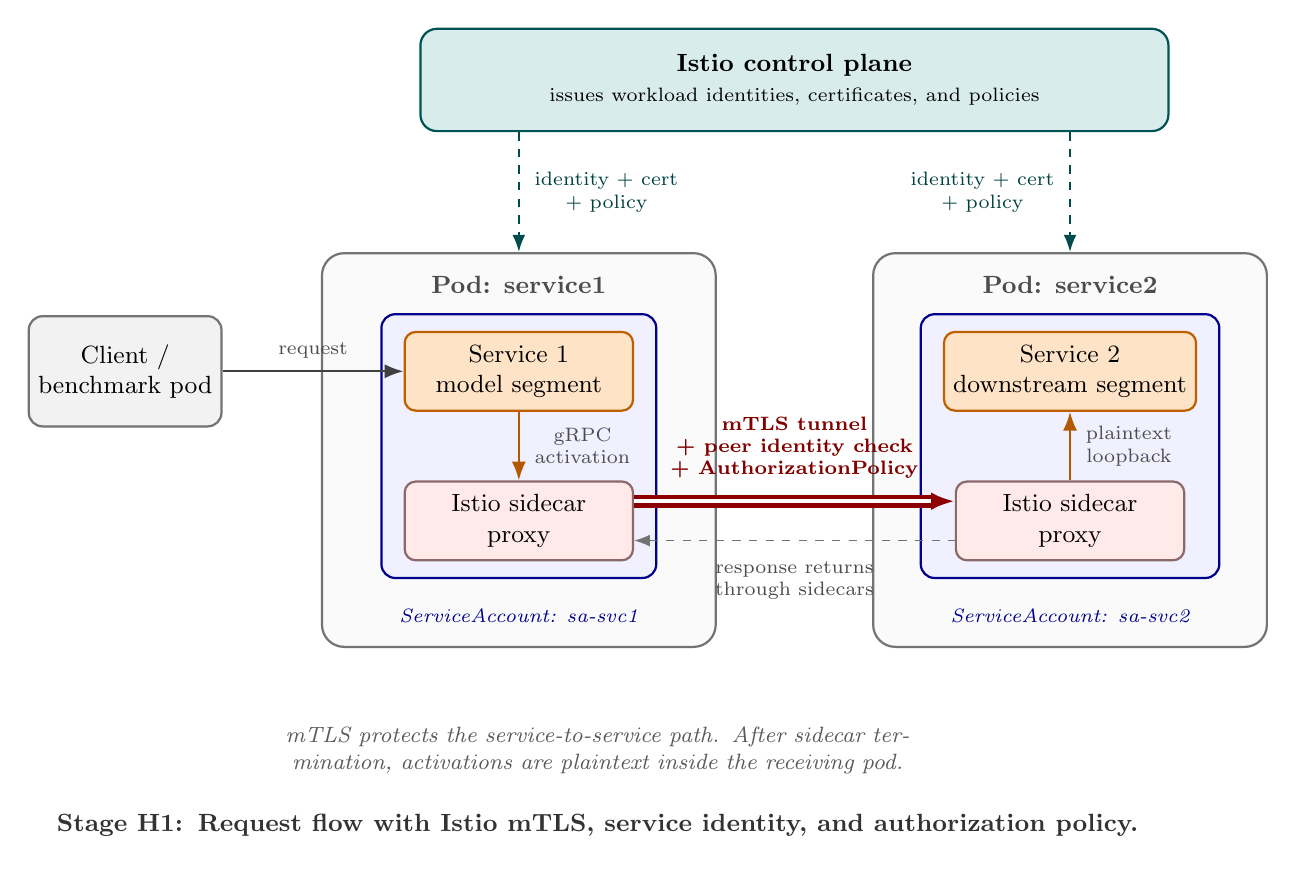
\begin{tikzpicture}[
    font=\small,
    workload/.style={
        draw=blue!55!black,
        fill=blue!6,
        rounded corners=5pt,
        thick,
        inner xsep=8pt,
        inner ysep=6pt
    },
    podbox/.style={
        draw=black!55,
        fill=black!2,
        rounded corners=8pt,
        thick,
        minimum width=5.0cm,
        minimum height=5.0cm,
        inner sep=0pt
    },
    app/.style={
        draw=orange!75!black,
        fill=orange!22,
        rounded corners=4pt,
        minimum width=2.9cm,
        minimum height=1.0cm,
        align=center,
        thick
    },
    sidecar/.style={
        draw=pink!55!black,
        fill=pink!35,
        rounded corners=4pt,
        minimum width=2.9cm,
        minimum height=1.0cm,
        align=center,
        thick
    },
    controlplane/.style={
        draw=teal!65!black,
        fill=teal!15,
        rounded corners=6pt,
        minimum width=9.5cm,
        minimum height=1.3cm,
        align=center,
        thick
    },
    client/.style={
        draw=black!55,
        fill=black!5,
        rounded corners=5pt,
        minimum width=2.4cm,
        minimum height=1.4cm,
        align=center,
        thick
    },
    podplain/.style={
        -{Latex[length=2.4mm]},
        thick,
        draw=orange!70!black
    },
    mtlsarrow/.style={
        -{Latex[length=3mm]},
        ultra thick,
        draw=red!55!black,
        double,
        double distance=1.5pt
    },
    identityarrow/.style={
        -{Latex[length=2.2mm]},
        thick,
        dashed,
        draw=teal!60!black
    },
    returnarrow/.style={
        {Latex[length=2mm]}-,
        thin,
        dashed,
        draw=black!55
    },
    requestarrow/.style={
        -{Latex[length=2.4mm]},
        thick,
        draw=black!75
    },
    labeltext/.style={
        font=\scriptsize,
        text=black!70,
        align=center
    },
    salabel/.style={
        font=\scriptsize\itshape,
        text=blue!55!black,
        align=center
    }
]

% --- Control plane (top) ---------------------------------------------------
\node[controlplane] (cp) at (3.5, 4.6)
    {\textbf{Istio control plane}\\
     \scriptsize issues workload identities, certificates, and policies};

% --- Pod 1 (service1) -----------------------------------------------------
\node[app]     (s1app)   at (0, 0.9)  {Service 1\\model segment};
\node[sidecar] (s1proxy) at (0, -1.0) {Istio sidecar\\proxy};

\begin{pgfonlayer}{background}
    \node[podbox] (col1) at (0, -0.1) {};
    \node[workload, fit=(s1app)(s1proxy)] (wl1) {};
\end{pgfonlayer}

\node[font=\small\bfseries, text=black!70, anchor=north]
    at ($(col1.north)+(0,-0.18cm)$) {Pod: service1};
\node[salabel, anchor=south]
    at ($(col1.south)+(0,0.20cm)$) {ServiceAccount: \textit{sa-svc1}};

% --- Pod 2 (service2) -----------------------------------------------------
\node[app]     (s2app)   at (7.0, 0.9)  {Service 2\\downstream segment};
\node[sidecar] (s2proxy) at (7.0, -1.0) {Istio sidecar\\proxy};

\begin{pgfonlayer}{background}
    \node[podbox] (col2) at (7.0, -0.1) {};
    \node[workload, fit=(s2app)(s2proxy)] (wl2) {};
\end{pgfonlayer}

\node[font=\small\bfseries, text=black!70, anchor=north]
    at ($(col2.north)+(0,-0.18cm)$) {Pod: service2};
\node[salabel, anchor=south]
    at ($(col2.south)+(0,0.20cm)$) {ServiceAccount: \textit{sa-svc2}};

% --- Client / benchmark pod (far left) -----------------------------------
\node[client] (client) at (-5.0, 0.9) {Client /\\benchmark pod};

% --- Control plane to sidecars (identity + cert + policy) -----------------
\draw[identityarrow]
    (cp.south -| col1.north) --
    node[labeltext, right=2pt, text=teal!50!black]
        {identity + cert\\+ policy}
    (col1.north);
\draw[identityarrow]
    (cp.south -| col2.north) --
    node[labeltext, left=2pt, text=teal!50!black]
        {identity + cert\\+ policy}
    (col2.north);

% --- Client request into Service 1 ----------------------------------------
\draw[requestarrow]
    (client.east) --
    node[labeltext, above=1pt] {request}
    (s1app.west);

% --- gRPC activation inside Pod service1 (app -> sidecar) -----------------
\draw[podplain]
    (s1app.south) --
    node[labeltext, right=2pt] {gRPC\\activation}
    (s1proxy.north);

% --- mTLS hop (sidecar 1 -> sidecar 2), slight upward offset --------------
\draw[mtlsarrow]
    ([yshift=2.5mm]s1proxy.east) --
    node[labeltext, above=4pt,
         text=red!50!black, font=\scriptsize\bfseries,
         text width=3.6cm]
        {mTLS tunnel\\+ peer identity check\\+ AuthorizationPolicy}
    ([yshift=2.5mm]s2proxy.west);

% --- Return arrow (sidecar 2 -> sidecar 1), slight downward offset --------
\draw[returnarrow]
    ([yshift=-2.5mm]s1proxy.east) --
    node[labeltext, below=4pt, text width=4cm]
        {response returns\\through sidecars}
    ([yshift=-2.5mm]s2proxy.west);

% --- Plaintext loopback inside Pod service2 (sidecar -> app) --------------
\draw[podplain]
    (s2proxy.north) --
    node[labeltext, right=2pt] {plaintext\\loopback}
    (s2app.south);

% --- Note below the figure ------------------------------------------------
\node[font=\footnotesize\itshape, text=black!65,
      align=center, anchor=north, text width=14cm]
    at (1, -3.5)
    {mTLS protects the service-to-service path.
     After sidecar termination, activations are plaintext
     inside the receiving pod.};

% --- Caption --------------------------------------------------------------
\node[font=\small\bfseries, text=black!80,
      align=center, anchor=north, text width=14cm]
    at (1, -4.6)
    {Stage~H1: Request flow with Istio mTLS, service identity,
     and authorization policy.};

\end{tikzpicture}
\end{document}
